\section{Four dimensions and the formula for the gap}
\label{sec:fourdim}

\begin{figure*}[t]
\centering
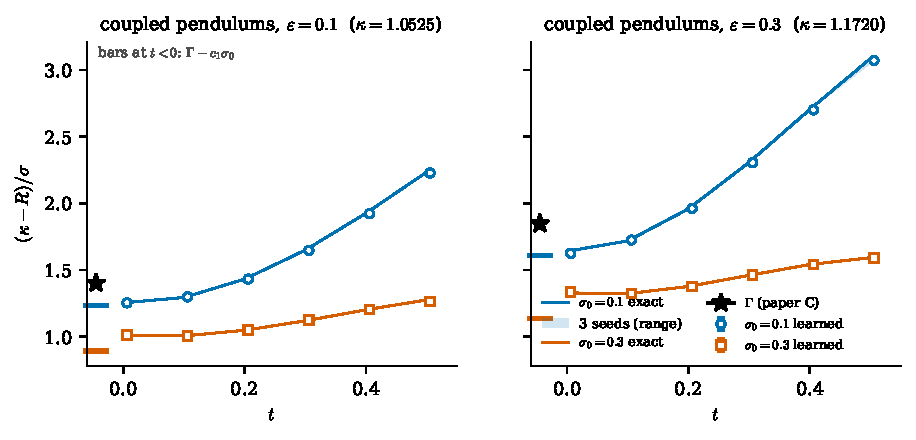
\includegraphics[width=0.9\textwidth]{figures/fig3_learned_4d.pdf}
\caption{Coupled pendulums, Eq.~\eqref{eq:coupled}: learned (symbols) and exact (lines) margins for $0 \leq t \leq 0.5$ at $r = \kappa$. Stars: $\Gamma$, the $\sigma \to 0$ limit of the best Gaussian state~\cite{namba2026many}; bars at $t<0$: $\Gamma - c_1\sigma_0$, the same with its finite-resolution correction. Shaded: range over three training seeds ($\varepsilon = 0.3$, $\sigma_0 = 0.1$).}
\label{fig:learned4d}
\end{figure*}

\begin{observation}
\label{obs:4d}
For $\varepsilon = 0.1$, $0.3$ and $\sigma_0 = 0.1$, $0.3$, the learned margin agrees with the exact margin to within $1.41\%$ at all 24 points, 21 of them inside the error band.
\end{observation}

The comparison is shown in Fig.~\ref{fig:learned4d}. The largest difference, $-1.41\%$, is again at $t = 0$, where the state is sharpest. Three networks trained with different seeds ($\varepsilon = 0.3$, $\sigma_0 = 0.1$) give margins whose standard deviation is $0.1$--$0.5\%$ and whose range is $0.2$--$1.0\%$ of the margin, comparable to the error band.

\begin{table}[t]
\caption{Four dimensions at $t = 0$: the margin of the $W = 3$ state, exact and learned, against the formula of Ref.~\cite{namba2026many}. $\Gamma - c_1\sigma_0$ includes the finite-resolution correction.}
\label{tab:fourdim}
\begin{ruledtabular}
\begin{tabular}{cccccc}
$\varepsilon$ & $\sigma_0$ & $\Gamma$ & $\Gamma - c_1\sigma_0$ & exact & learned \\
\hline
$0.1$ & $0.1$ & $1.4025$ & $1.2325$ & $1.2615$ & $1.2536$ \\
$0.3$ & $0.1$ & $1.8475$ & $1.6095$ & $1.6484$ & $1.6252$ \\
$0.1$ & $0.3$ & $1.4025$ & $0.8925$ & $1.0106$ & $1.0136$ \\
$0.3$ & $0.3$ & $1.8475$ & $1.1335$ & $1.3340$ & $1.3347$ \\
\end{tabular}
\end{ruledtabular}
\end{table}

\emph{Against the formula.} Table~\ref{tab:fourdim} compares the margin at $t = 0$ with the formula for the gap. At $\sigma_0 = 0.1$ the learned margin lies within $1.0$--$1.7\%$ of $\Gamma - c_1\sigma_0$, and the exact margin of the $W = 3$ state within $2.3$--$2.4\%$; both are $10$--$12\%$ below $\Gamma$ itself. The finite-resolution correction is therefore visible to the learned score. At $\sigma_0 = 0.3$ the linear correction overshoots: the margins lie $13$--$18\%$ above $\Gamma - c_1\sigma_0$, as expected when $c_1\sigma_0$ is no longer small compared with $\Gamma$. A network that never saw the formula thus reads a margin consistent with a matrix formula derived from the potential alone.

\emph{Entropy measured directly.} For $\varepsilon = 0.3$, $\sigma_0 = 0.1$, $r = \kappa$, we measured the entropy increase over five intervals of length $0.1$ with the nearest-neighbour estimator (Fig.~\ref{fig:entropy}, right). The prediction from the learned networks, Eq.~\eqref{eq:Sdot} integrated with the divergence form, agrees with the exact prediction to within $0.5\%$. The direct measurement brackets both: applied to the raw samples it is $0.5$--$6\%$ above, and applied after a global linear whitening it is $1$--$3\%$ below. The nearest-neighbour estimator is biased for a strongly anisotropic density with few neighbours per unit of the thin direction; whitening removes the anisotropy of the bulk but not that of the curved tails, which is why the two versions straddle the prediction. In two dimensions, where the bias is negligible, the measurement agrees with the exact entropy over all 30 intervals to within three standard errors, mostly within one (Fig.~\ref{fig:entropy}, left).

\begin{figure*}[t]
\centering
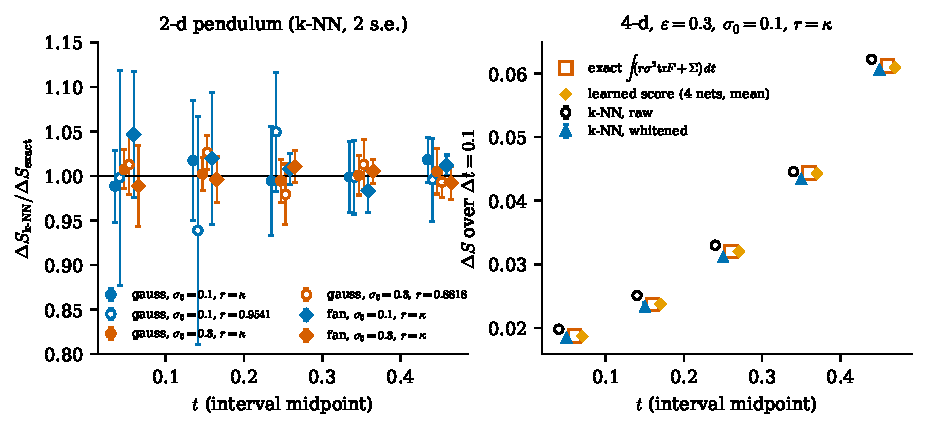
\includegraphics[width=0.9\textwidth]{figures/fig6_entropy.pdf}
\caption{Entropy increase measured directly with the Kozachenko--Leonenko estimator ($k = 4$), with no score. Left: pendulum, ratio of the measured to the exact increase over intervals of length $0.1$ (two standard errors), for $r = \kappa$ and for $r$ inside the band. Right: coupled pendulums, $\varepsilon = 0.3$, $\sigma_0 = 0.1$, $r = \kappa$: exact prediction $\int(r\sigma^2\tr F + \Sigma)\,dt$, the same from the learned networks (mean of four), and the nearest-neighbour measurement on raw and on whitened samples.}
\label{fig:entropy}
\end{figure*}
